% This file is part of the QuasarVariability project
% Copyright 2013 David W. Hogg (NYU) and any other authors.

\documentclass[letterpaper,12pt,preprint]{aastex}

\newcommand{\project}[1]{\textsl{#1}}
\newcommand{\sdss}{\project{SDSS}}
\newcommand{\lsst}{\project{LSST}}
\newcommand{\ptf}{\project{PTF}}
\newcommand{\panstarrs}{\project{PanSTARRS}}
\newcommand{\given}{\,|\,}
\newcommand{\transpose}[1]{{#1}^{\mathsf{T}}}
\newcommand{\inverse}[1]{{#1}^{-1}}

\begin{document}

\title{Probabilistic models for heterogenous multi-band multi-epoch
  photometry of time-variable quasars.}
\author{DM, EP, DWH, HWR, NH, DFM, others}

\begin{abstract}
Recent projects have built likelihood functions for stochastically
variable quasar light-curves based on Gaussian Processes.  There are
successful models based on damped random walks and also power-law
structure functions, but all of the models effectively assume that the
data are coming from a single photometric bandpass.  Here we generalize
these models so that they can accept data from multiple different
photometric bandpasses, whether or not the data taken through the
different bandpasses are taken simultaneously (as in \sdss) or with
large time lags (as with \panstarrs\ and \lsst).  The model naturally
captures luminosity-correlated color changes.  We test the models on
data from \sdss\ \project{Stripe 82}, in which multi-epoch data was
taken effectively simultaneously in five photometric bandpasses, and
we also test the models on data subsamples in which there are no
simultaneous measurements.  We find that we can infer
structure-function parameters in either case, and that the model can
be used to separate stars and quasars.  We also show that we can infer
time-dependent (and mean) quasar colors, even when a source shows
substantial variability but has not ever been measured simultaneously
in different bands.
\end{abstract}

\keywords{
  this ---
  that ---
  quasars
}

\section{Introduction}

Why what has been done with \sdss\ and \ptf\ data won't be sufficient
for \panstarrs\ and \lsst.

Macleod, et. al. 2010 - ``Modeling the Time Variability of SDSS Stripe
82 Quasars as a Damped Random Walk'': This paper shows the high degree
of agreement between the Damped Random Walk model and quasars from
stripe 82. They use a standard covariance matrix of $V = a^2 \exp
\left (-|\frac{\Delta t}{\tau}|\right)$. They are also more interested
in overall properties of quasars, not identifying individual
objects. As far as I can tell, they do multi-band fitting, but only in
the sense that stripe 82 is simultaneous.

Zu, et. al. 2012 - ``Is Quasar Optical Variability a Damped Random
Walk'': This paper looks at the time sensitive effects of the fitting
quasar variability with damped random walks. They also use a standard
covariance function where
\begin{eqnarray}
S_{DRW}=\sigma^2\exp\left(-\frac{\Delta t}{\tau}\right)
\end{eqnarray}
,but change it at small time scales in a piecewise
manner to test for deviations on short and long timescales. The data
used in this method is taken from OGLE and only occurs in the i-band.
The results show that on short timescales of a few months, there seems
to be a characteristic cutoff timescale and stronger correlations than
the DRW model. On long timescales of a few years or more, the
light-curves seem to be well-defined by the DRW model, but the
precision becomes limited by the length of the light-curves.

Brewer, 2013. (personal communication): Brewer uses the Gaussian
Process to measure time delays in gravitationally lensed quasars. The
data used for this Gaussian Process is from all images, not just one
image at a time. The structure of the covariance matrix varies with
parameters. Generally, the elements of the covariance matrix are given
by a function of the form:
\begin{eqnarray}
C_{ij}=\sigma^2 \exp\left[-\frac{|t_i-t_j|}{L}\right],
\end{eqnarray}
where $\sigma$ and $L$ are functions of time for quasar variability or
a microlensing signal specific to the image. For microslensing
signals, the exponential term is raised to a power $\alpha$, which is
a smoothness parameter for microlensing signals. Though it is not
explicityly stated, I assume that the images are taken in certain
bandpasses, from which all magnitudes are combined and used as one
vector of measured magnitudes.

Schmidt et al. 2010 - ``Selecting Quasars by their Intrinsic
Variability'': This method for selecting quasars is carried out by
parametrizing single-band variability using a power-law model for the
light-curve structure function with an amplitude, $A$ and a power law
index, $\gamma$. The power-law model for the structure function is:
\begin{eqnarray}
V_{mod}(\Delta t_{i,j}|A,\gamma)=A\left(\frac{\Delta t_{i,j,}}{1
  yr}\right)^{\gamma}.
\end {eqnarray}
The power-law model is fitted with given data where $\Delta m_{i,j,}$
is the difference in magnitude of light-curve points and $\Delta
t_{i.j}$ is the separation between the magnitudes. The likliehood
function is then:
\begin{eqnarray}
{\cal L}(A|\gamma)= \prod_{i,j} L_{i,j},
\end{eqnarray}
and the elements $L_{i,j}$ are
\begin{eqnarray}
L_{i,j}=\frac{1}{\sqrt{2\pi V_{eff,ij}^2}}\exp\left(-\frac{\Delta
  m_{i,j}^2}{2V_{eff,ij}^2} \right).
\end{eqnarray}
The effective, observed variability is
\begin{eqnarray}
V_{eff,ij}^2=V_{mod}(\Delta t_{ij}|A,\gamma)^2+ (\sigma_i^2 +
\sigma_j^2),
\end{eqnarray} 
where $\sigma_i$ and $\sigma_j$ are the photometric errors. They
utilize Stripe 82 data to select extensive, complete and pure quasar
samples.

Butler \& Bloom, 2011 - ``Optimal Time-Series Selection of Quasars'':
Butler and Bloom present an optimal selection of potential quasars in
the range of redshift, 2.5 $<$ z $<$ 3 using time series observations
in a single photometric bandpass. This range of redshifts is typically
difficult to use color selection methods on for identifyig
quasars. Using the damped random walk model presented by Kelly et
al. 2009, Butler and Bloom parametrize the quasar structure function
in Stripe 82 as a function of observed brightness. The covariance
matrix used is
\begin{eqnarray}
C_{ij}=\sigma_i^2 \Delta_{ij} + \frac{1}{2}\hat{\sigma}^2 \tau_0 \exp
\left(-\frac{\tau_{ij}}{\tau_0}\right),
\end{eqnarray}
where $\sigma_i$ is the measurement uncertainty, $\tau_{ij}=t_i=t_j$
is the time between measurements, $\tau_0$ is an exponential damping
timescale in units of days, and $\hat{\sigma}^2$ is the intrinsic
variance between magnitude observations on timescales of about 1 day.

Brewer \& Stello, 2009 - ``Gaussian Process Modeling of Asteroseismic
Data'': Brewer \& Stello use a probabilistic model to infer the
frequencies and amplitudes of stellar oscillation modes assuming there
is some periodic, quasi-sinusoidal oscillation in subgiant and red
giant stars. The apply a damped oscialltion to the time series of
simulated data and then to real data for the red giant star $\xi$
Hydrae to recover its mode lifetime. They use a typical covariance
function multilpied by a cosine term to determing the elements of the
covariance matrix:
\begin{eqnarray}
C(\Delta t)= A^2 \exp \left( -\frac{|\Delta t|}{\tau'}\right ) \cos (2
\pi \nu \Delta t).
\end{eqnarray}
$A$ is the oscillation amplitude, $\nu$ is the oscillation frequency
and $\tau$ is the decay timescale.

Kelly et al., 2009 - ``Are the Variations in Quasar Optical Flux
Driven by the Thermal Fluctuations?'': This paper models light curves
as continuous stochastic processes which provide natural estimates for
timescale and amplitude. A continuous autoregressive process where
$A$, $\tau$ and $\sigma$ are free parameters is used to measure the
light-cruves for data taken from the MACHO survey, PG Quasars and
Seyfert galaxies. Light-curves that follow a power spectrum
proportional to $1/f^2$ are suggestive of random walks and stochstic
timescales. The following equations describes the autoregressive
process:
\begin{eqnarray}
dX(t)=\frac{1}{\tau}X(t)dt + \sigma\sqrt{dt}\epsilon(t)+bdt
\tau,\sigma,t > 0.
\end{eqnarray}
The variance for $X(t)$ is the following given $X(s)$ where s $<$ t:
\begin{eqnarray}
Var(X(t)|X(s))=\frac{\tau \sigma^2}{2}\left [ 1-e^\frac{-2\Delta
    t}{\tau}\right].
\end{eqnarray}
Only one bandpass is used in this study. (Not sure that I did this
paper justice or if this is the math that we want to include from it)

Bovy, HWR, et al.(personal communication) - ``Broadband photometric
reverberation mapping'': Data from Stripe 82 and light-curves
downloaded from SDSS DR7 CAS are used to show that all photometry can
be modeled as linear combinations of the light-curves shifted by
delays due to the delayed response of emission lines to the continuum flux.
Using the g-band with a broad emission line and the r-band with a
continuum flux only, where the r-band flux varies linearly with the
g-band, covariance functions for the contiuum model can be written as:
\begin{eqnarray}
C^{cc}_{rr}(\Delta t)=s^2C^{cc}_{gg}(\Delta t),
\end{eqnarray} 
\begin{eqnarray}
C^{cc}_{gr}(\Delta t)=s C^{cc}_{gg}(\Delta t),
\end{eqnarray}
where $s$ is the linearly scale factor between the g and r-band and
the superscript $^c$ represents continuum contributions to the
flux. The time delay between emission lines and continuum flux is
described by a one-dimensional transfer function, which eventually
allows the fluxes in the g and r-bands to be written in terms of
continuum and emission line covariance matrices.  Continuum
variability in the g-band is then modeled by a Gaussian process, using
a power-law structure function, to predict the magnitude and relative
flux variability. The structure function power-law is a cut-off power
law:
\begin{eqnarray}
V(\Delta t)\equiv1/2\langle((f(t)-f(t+\Delta t))^2\rangle \equiv
\frac{1}{2} A^2 \left(\frac{\Delta t}{1 yr}\right)^\gamma,
\end{eqnarray}
where $f$ is flux at a given time.

Hernitschek, N. (Masters Thesis, University of Heidelberg \& MPIA) -
``Estimating Black Hole Masses in Hundreds of Quasars'':

This study aims to measure the broad-line region time delay due to
finite light travel time. Measuring the time delay also provides
insight on the BLR size, structure and with knowledge of the BLR
velocities can used to infer black hole masses. A stochastic
reverberation mapping technique is developed to test on many quasars
in the SDSS Stripe 82 data, which contains flux measurements for about
60 epochs, but initial testing of this technique is first applied to
mock light-curves. Two structure functions are evaluated on the mock
light-curves in this analysis, one follows a power-law and the other
is a damped random walk model. Their mathematical representations are:
\begin{eqnarray}
V(t_{ij})=A^2 \left(\frac{\Delta t_{ij}}{1 yr}\right) ^\gamma,
\end{eqnarray} and
\begin{eqnarray}
C_{ij}=\frac{\omega ^2}{2} \exp \left(- \frac {|\Delta t_{ij}|}{\tau}\right).
\end {eqnarray}
In the power-law structure function, $A$ and $\gamma$ are the
dimensionless parameters described in Schmidt et al., 2010. For the
damped random walk model, the $\omega ^2$ is the intrinsic variance of
the data. For all light-curve assessments, only one bandpass is
observed at a time.

MacLeod et al., 2012 - ``A Description of Quasar Variability Measured
Using Repeated SDSS and POSS Imaging'': MacLeod et al. provides a
statistical interpretation of continuum quasar variability in the
optical range. They use SDSS and POSS data with a damped random walk
model to explain the ensemble variability for quasars that are not in
S82, such as those quasars with exponential distributions of large
magnitude changes. The damped random walk model proves to be accurate
for time scales of 5-2000 days, which allows this model to be used to
predict quasar contamination in transient surveys. The ensemble
structure function is given by the weighted structure function of all
individual quasars structure functions:
\begin{eqnarray}
SF(\Delta t)= \int d\tau dSF_{\infty} \frac{d^2n}{ d\tau dSF_{\infty}}
SF(\Delta t| \tau,SF_{\infty})_{qso},
\end{eqnarray} 
where $ SF(\Delta t| \tau,SF_{\infty})_{qso}$ is the structure
function for a quasar at some time $\Delta t$ with DRW parameters
$\tau$ and $SF_{\infty}$ given by
\begin{eqnarray}
 SF(\Delta t| \tau,SF_{\infty})_{qso}=SF_{\infty}(1-e^{-|\Delta
   t|/\tau})^{1/2}.  
\end{eqnarray}
Note that $SF(\Delta t)_{qso}$ is the standard
 deviation in magnitude difference, $\Delta m$, for some $\Delta t$ and is related
 to the standard deviation of magnitudes by $SF(\Delta
 t)_{qso}=\sqrt{2}\sigma_m$.



\section{The model}

In our language, a ``model'' is a likelihood function---a function
equal to or proportional to a pdf in data space for the data given
parameters---and a set of prior pdfs for some or all of those
parameters.  For this project, the ``data'' for one quasar comprise a
set of $N$ observed magnitudes $m_n$.  About each data point we have
various bits of (assumed correct) meta data: We know the time $t_n$ at
which each measurement was made.  We know the astronomical bandpass
$b_n$ through which the measurement was made.  The bandpass variable
$b_n$ can only take on one of a small number of possible integer
values (5 in the case of \sdss\ and \panstarrs, each of which observe
in 5 substantially distinct bandpasses).  We also know the variance
$\sigma_n^2$ of the noise contribution to the measurement $m_n$, which
we will assume is not only correct but also represents the variance of
a Gaussian pdf for the noise.  That is, we are assuming Gaussian
uncertainties of known (though heteroskedastic) variance.

To generate the likelihood function we use here, we make
use of a Gaussian Process formulation for stochastic quasar
variability; this formulation can encompass damped random walks
and also power-law structure functions (and indeed many other kinds of
continuous stochastic variability).  The unusual aspect of the model
we use here is that the Gaussian Process is not in any particular band
but instead in an ersatz fiducial band which can be scaled and shifted
onto the particular bands.  This permits simultaneous treatment of
multiple bands, even when the multiple bands are not observed
simultaneously.  The key idea is that the ersatz band is a latent
variable---it is never directly observed; only the scaled and shifted
versions are observed, and even these are only observed in the
presence of substantial measurement noise.

In the damped random walk model, without loss of generality (the real
photometric measurements will be scaled and shifted to match the
latent ersatz basis), the ersatz lightcurve can be described with a
zero-mean and unit-characteristic-variance Gaussian Process.  That is,
the prior pdf for a set of $N$ ersatz ``magnitudes'' $q_n$ that are
instantiated at times $t_n$ is just
\begin{eqnarray}
p(q) &=& N(q\given 0,V)
\\
\transpose{q} &\equiv& [q_1, q_2, \cdots , q_N]
\\
V_{nn'} &=& \exp -\frac{|t_n - t_{n'}|}{\tau}
\quad ,
\end{eqnarray}
where $N(x\given\mu,V)$ is the multivariate normal for column vector
$x$ given mean vector $\mu$ and general variance tensor $V$, $q$ is
the $N$-dimensional column vector made up of all the latent ersatz
magnitudes $q_n$, $0$ is not zero but the $N$-dimensional
generalization of zero, $V$ is a $N\times N$ symmetric positive
definite matrix with elements $V_{nn'}$, and $\tau$ is the
decorrelation time of the random walk.  Some draws from this kind of
Gaussian Process are shown in \figurename~\ref{fig:qdraws}; it is a
model of stochastic variation with controlled correlation properties.

The pdf for an individual measurement $m_n$ given its meta data and a
value for the corresponding latent ersatz magnitude $q_n$ is found by
shifting and scaling the latent magnitude and adding Gaussian noise.
This makes a single-datum likelihood
\begin{eqnarray}
p(m_n\given q_n,b_n,\sigma_n^2) &=& N(m_n\given a(b_n) * q_n + \mu(b_n), \sigma_n^2)
\quad ,
\end{eqnarray}
where $a(b)$ is a scale appropriate to photometric bandpass $b$,
$\mu(b)$ is an offset or mean appropriate to bandpass $b$, and there
is one value of $a(b)$ and one value of $\mu(b)$ for each possible
value of the bandpass $b$.  Because everything is Gaussian, the latent
ersatz magnitudes never have to be explicitly inferred individually;
they can all be marginalized out analytically.

We generate our individual band amplitudes and time shifts using
\begin{eqnarray}
a(b_n) &=& a_r(\frac{\lambda(b_n)}{\lambda(b_r)})^\alpha
\\
\Delta(b_n) &=& \Delta_r(\frac{\lambda(b_n)}{\lambda(b_r)})^\gamma
\quad ,
\end{eqnarray}
where here $\alpha$ is our exponent for the amplitudes, and $r$ is the band we have chosen to work in as our base band. $\lambda$ is the respective wavelength for each band. $\gamma$ here is our exponent for the time shifts for each band. We considered a model where the $\tau$ values for each band would vary similiary, but found that it resulted in a non positive definite kernel. We also decided to fix $\gamma$ to one. [why? -dm]

This marginalization (to remove all explicit mention of the ersatz
variable $q$) leads to the following very simple covariance function
for the data:
\begin{eqnarray}
p(m) &=& N(m\given \mu,V)
\label{eq:likestart}
\\
\transpose{m} &\equiv& [m_1, m_2, \cdots , m_N]
\\
\transpose{\mu} &=& [\mu(b_1), \mu(b_2), \cdots , \mu(b_N)]
\\
V_{nn'} &=& a(b_n)\,a(b_{n'})\,\exp -\frac{|t_n - t_{n'}+\Delta(b_n) - \Delta(b_{n'})|}{\tau} + \sigma_n^2\,\Delta_{nn'}
\label{eq:likeend}
\quad ,
\end{eqnarray}
where $m$ is a column vector of all the observations (from all bands),
$\mu$ is a column vector of all the means, with each mean value in the
vector drawn from the list of five means $\mu(b)$ but appropriately
for the data point in question, the rows and columns of the variance
tensor $V$ have been multiplied by the scales $a(b)$ appropriate for
the relevant observations, and there is an additional term
$\sigma_n^2$ added only to the diagonal elements to model the
measurement noise variance.  This model is very rigid, in that the
bandpasses are tightly tied to one another, but also very flexible, in
that the quasar can have any mean color and that color can change
(deterministically) as it brightens (as is observed [HOGG CITE]).
Some draws from this multi-band damped-random-walk Gaussian Process
are shown in \figurename~\ref{fig:mdraws}

The equations~(\ref{eq:likestart}) through (\ref{eq:likeend})
provide a method for computing the probability of any data set (any
set of observed magnitudes $m_n$) given meta data (times $t_n$,
bandpasses $b_n$, observational uncertainties $\sigma_n^2$) and
parameters $a(b)$ (five numbers), $\mu(b)$ (five numbers), and $\tau$.
The probability of the observed data given parameters is the
\emph{likelihood function}.  Thus we can bring the whole machinery of
probabilistic inference (likelihood optimization, posterior sampling)
to the problem.  Also, because both the process is Gaussian and the
noise is (assumed to be) Gaussian, it is trivial to make prior draws
of expected data, and also make \emph{conditional predictions} for new
data $\tilde{m}_k$ at $K$ times $t_k$ taken through bandpasses $b_k$ with
expected uncertainties $\sigma_k^2$ given the data in hand (which are
at $N$ times $t_n$):
\begin{eqnarray}
p(\tilde{m}|m) &=& N(\tilde{m}|\tilde{\mu},\tilde{V})
\\
\transpose{\tilde{m}} &\equiv& [\tilde{m}_1, \tilde{m}_2, \cdots , \tilde{m}_K]
\\
\tilde{\mu} &=& \nu + X\cdot\inverse{V}\cdot [m - \mu]
\\
\tilde{V} &=& Y - X\cdot\inverse{V}\cdot\transpose{X}
\\
\transpose{\nu} &=& [\mu(b_1), \mu(b_2), \cdots , \mu(b_K)]
\\
X_{kn} &=& a(b_k)\,a(b_n)\,\exp -\frac{|t_k - t_n + \Delta(b_k) - \delta(b_n)|}{\tau}
\\
Y_{kk'} &=& a(b_k)\,a(b_{k'})\,\exp -\frac{|t_k - t_{k'}+\Delta(b_k) - \Delta(b_{k'})|}{\tau} + \sigma_k^2\,\Delta_{kk'}
\quad ,
\end{eqnarray}
where $\tilde{m}$ is the column vector of conditional predictions,
$\tilde{\mu}$ and $\tilde{V}$ are a conditional mean vector and a
conditional variance tensor, (temporary) mean vector $\nu$ is
$K$-dimensional, and the matrices $V$, $X$, and $Y$ are $N\times N$,
$K\times N$, and $K\times K$ respectively.  Vectors $m$ and $\mu$ and
matrix $V$ are defined above in equations~(\ref{eq:likestart}) through
(\ref{eq:likeend}).  These conditional predictions depend on the
Gaussian Process parameters.  They represent an adjusted Gaussian
Process, adjusted to ``go through'' (or at least near) the existing
data.  We show an example of conditional predictions in
\figurename~\ref{fig:conditional}

\section{Inference}

We applied an iteratively-reweighted least squares procedure on the data before proceeding with the inference. To generate this, we fixed the parameters of our models to nominal values, and then updated the $\sigma$ terms according to the following rule: \begin{equation} \sigma_{new} = \sigma_{old} \sqrt{Q^2+(\frac{mags-condmags}{\sigma_{old}^2+condvars})^2}\end{equation}

For each mean hyperparamater, we used a Gaussian centered at $20$ with a variance of $10$. For our $\log(a_r)$ hyperparameter we used a prior of a Gaussian centered at $-1$ with a variance of $1$. For $\alpha$ our prior was a Gaussian centered at $-1$ and a variance of $.25$. For $\log(\tau)$ we used a Gaussian centered at $5$ and a variance of $2$. For $\delta_r$ we used a Gaussian with a mean of $0$ and a variance of $1$. For $\gamma$ we used a Gaussian with a mean of $-1$ and a variance of $.25$. 


We used MCMC to sample our posterior distribution. For this, we used the emcee python package.

INSERT TRIANGE PLOT

INSERT MODEL COMPARISON


\section{Experiments}

\section{Discussion}

...Promise for \lsst...

...Caveats related to reverberation mapping...

%\acknowledgements
It is a pleasure to thank Zoubin Ghahramani (Cambridge) for posting a
very valuable Gaussian Process tutorial online.

\clearpage
\begin{figure}
~[DM + EP]~
\caption{Four draws from the damped random walk model for the latent
  variable $q$.  These draws are made with $a=0.75$~mag and
  $\tau=400$~d.\label{fig:qdraws}}
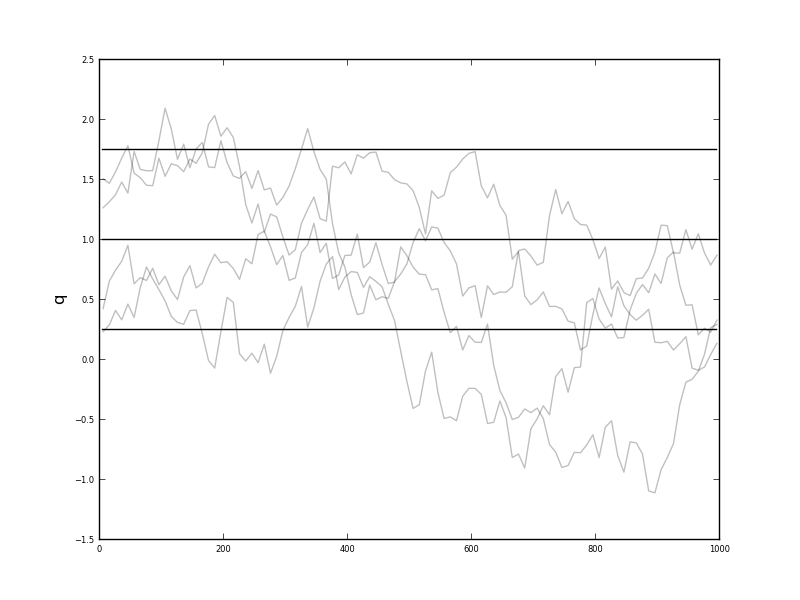
\includegraphics [width=\textwidth]{latentvar.png}
\end{figure}

\begin{figure}
~[DM + EP]~
\caption{Four draws from the multi-band damped random walk model in
  the five SDSS bands.  These draws are made with $a(b)=(0.85, 0.75,
  0.65, 0.55, 0.45)$~mag in the five bandpasses, $\mu(b)=$[DM+EP], and
  $\tau=400$~d.  The model is rigid in the sense that the five bands
  are all scaled replicas of one another.\label{fig:mdraws}}
\end{figure}

\begin{figure}
~[DM + EP]~
\caption{Example of conditional
  prediction... [DM+EP]\label{fig:conditional}}
\end{figure}

\end{document}
